

\section{Maps}
Maps were designed in a top-down view. The only limitation was that walls were perpendicular to floors. Everything could be done in 2D. A designed worked with only a few elements: \cw{VERTEX}\footnote{Vertices corrdinates were expressed with signed short integer [-32768, 32767]}, \cw{LINE}, \cw{SIDEDEF}, \cw{SECTOR}, and \cw{THING}.\\
\par
\drawing{doom_map_basics}{}

\par
A \cw{SECTOR} is an area surrounded by \cw{LINE}s with a specified floor height, floor texture, ceiling height, ceiling texture, and a light level. A sector could be concave, but lines could not cross each others.\\
\par
A \cw{LINE} could either be a solid wall or a portal between two \cw{SECTOR}s. The difference was in the number of \cw{SIDEDEF} associated with it. A wall had only one \cw{SIDEDEF} on its right side and is fully opaque. A portal had two \cw{SIDEDEF}s and can usually be seen though.\\
\par
A \cw{SIDEDEF} describe one side of a line. To accommodate walls and portals texturing it can have up to three textures. The middle texture is used by wall for the full area they cover. There was also a lower texture and an upper texture for portal connecting \cw{SECTOR}s with different ceiling/floor height. If the portal led to a sector with higher floor, the lower texture is used to render the "step". If the \cw{SECTOR} connects to a \cw{SECTOR} with lower ceiling, the upper texture is used to render the "down step". To help aligment with door and buttons, \cw{SIDEDEF} textures could also be offseted vertically and horizontally. \\
\par
A \cw{THING}s is must simpler in comparison. It only had one \cw{VERTEX} coordinate, an angle and an identifier telling its type. As the minimum a map must have one player spawning location \cw{THING}.\\

\cfullimage{doom_map.png}{Rendition of map shown in figure \ref{doom_map_basics}.}
\par
The resulting scene is ugly but the colors hopefully help to dissociate each elements. All \cw{LINE}s are walls except for \cw{E-B} which has two \cw{SIDEDEF}s and is therefore a portal. All walls use the \cw{BRIK} middle texture except for the portal which uses \cw{GRAY} for both top and bottom.\\
\par
\cw{SECTOR} \#0 uses a \cw{RED} floor texture and a \cw{WOOD} ceiling texture. The height of the floor is 20 and its ceiling is at 40. \cw{SECTOR} \#1 uses a \cw{BLUE} floor texture and a \cw{GREN} ceiling texture. Its floor is at 60 and ceiling at 60. Both sectors have the same light level (10).\\
\par
   Notice the portal \cw{E-B} which did not have a mid-texture but an upper and lower texture. These were used to draw the up-step and down-step to sector \#0.\\
\par
Also notice the wall \cw{D-E} which mid-texture vertical offset was not correctely set, resulting in a vertical tear when connecting with wall \cw{E-F}. Wall \cw{B-C} vertical offset was properly set and result in no visual artifact. None of the wall use an horizontal offset, however field is marked \cw{XOFF} to show its location.\\ 
\pagebreak



\subsection{Map Editor (DoomED)}
To harness the complexity of the map format, a new tool was created. The Doom map EDitor would be called \textbf{DoomED}. This is were \NeXT solution asserted the most impact. The high resolution of the display allowed a lot of real-estate showing small details and many widgets. The stability of NeXTSTEP allowed to never lose work while writing DoomED or creating a map.
The very design of Objective-C also had a tremendous influence. The language's message dispatching system no-op behavior when dereferencing a \cw{nullptr}\footnote{"Understanding the Objective-C Runtime".} created a fault forgiving environment where a feature would not work but did not crash either.\\
\par   
The killing feature was Application Builder which not only came with a full library of widgets but also allowed to create new one and connect them to the business logic instantly.\\
\par
\fullimage{doomed/DoomEd.png}
\par

The release of the source code in April 2015 allowed to pick inside. There is almost as much code as in the game engine (doom:32kloc, DoomED:20kcloc). Without the power of \NeXT the editor would have taken at least twice the same amount of time to make.\\
\par
\tcode{cloc_doomed.txt}
\par
DoomED was designed to be the "Adobe Illustrator" of doom maps where the designer simply drew line, selected sectors , and picked textures. A skilled map maker could complete a map in 20 minutes \fixme{citation needed}.\\
\par

\trivia{DoomED icon is an Imp. Upon startup a growling sound is played.}\\
\par
\fullimage{doomed/all_widgets.png}
\par


DoomED did not output data usable by the game engine directly. Instead it generated a text format output called \cw{DWD}. A header served as magic number which was followed by a list of lines listing sidedefs and a list of things. Sectors were inferred from line's ceiling/floor textures valus.\\
\par
\tcode{map.txt}
\par
DWD was designed with space efficiency in mind but rather to be easy to parse since it was processed by a tool called Node Builder.\\
\par
\cfullimage{props/tom.png}{Tom Halls, delighted next to his NeXTCube running DoomED.}
\par

\pagebreak





\section{Map Preprocessor (Node Builder)}
Map preprocessing was not something new at id. Since 1991, Wolfenstein 3D maps had been preprocessed to allow fast sound propagation. However with \doom, it had to be taken to a whole new level in terms of complexity and processing delay. The free form of the walls made the DDA\footnote{Digital differential analyzer, see Game Engine Black Book: Wolfenstein 3D} algorithm unusable. With the lose of DDA, gone were fast and cheap collision detection/wall sorting.\\
\par
To allow runtime to achieve an acceptable framerate, special optimized datastructures had to be generated. This was the task of 
\cw{doombsp}.\\
\par
 processes output from DoomED (XXX files) into XXX, XXX, and XXX. It was released very shorty after Doom shareware on April, 6th 1994. It is a small code base which was critical to the modding community since it enabled enthusiast to compile and inject their own maps into Doom.\\
\par
\tcode{cloc_doombsp.txt}
\par
\trivia{How long did it take to preprocess one map? All maps in Doom?}




\pagebreak
\par
\begin{figure}[H]
\centering
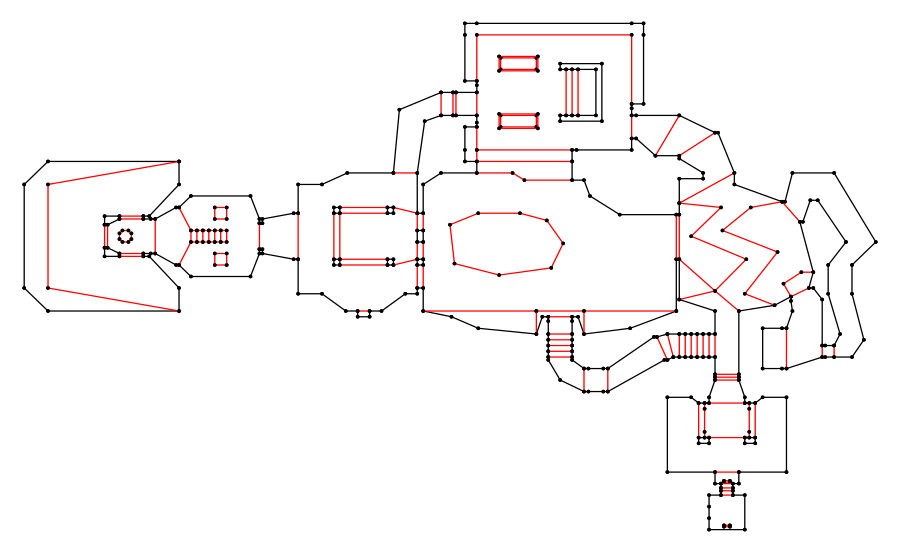
\includegraphics[width=\textwidth]{drawings/E1M1_lines.pdf}
\end{figure}
\par
The map as it is generated via the editor (DoomED) on NextStation.\\
\par
\begin{figure}[H]
\centering
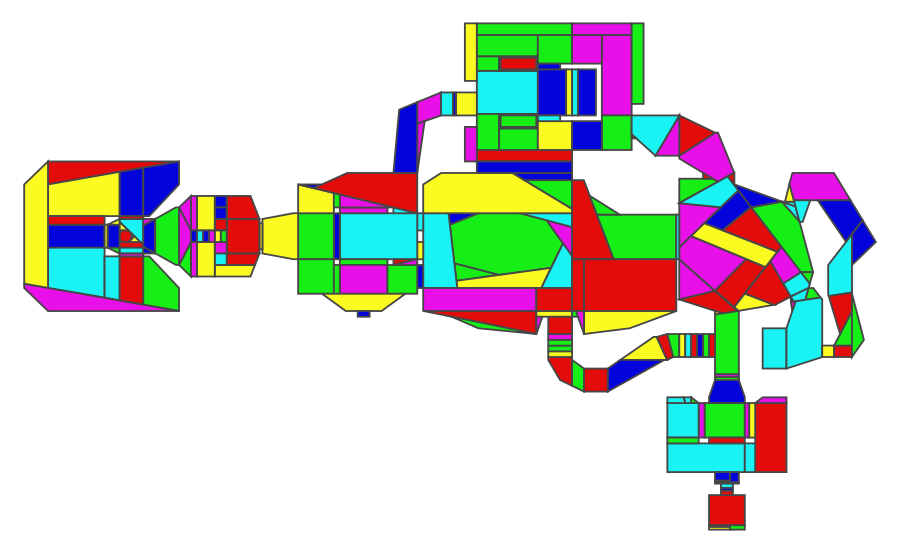
\includegraphics[width=\textwidth]{drawings/E1M1_fab.pdf}
\end{figure}
\par
Binary space partition. Slice all sectors into convex sub-spaces called subsectors.\\
\par
\begin{figure}[H]
\centering
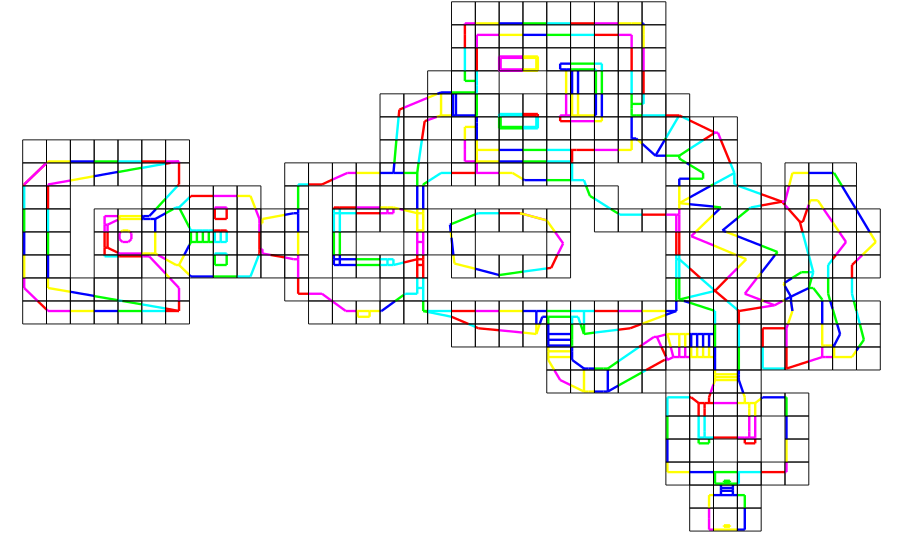
\includegraphics[width=\textwidth]{drawings/E1M1_blockmap.pdf}
\end{figure}
\par
Block based line index.\\
\par
\begin{figure}[H]
\centering
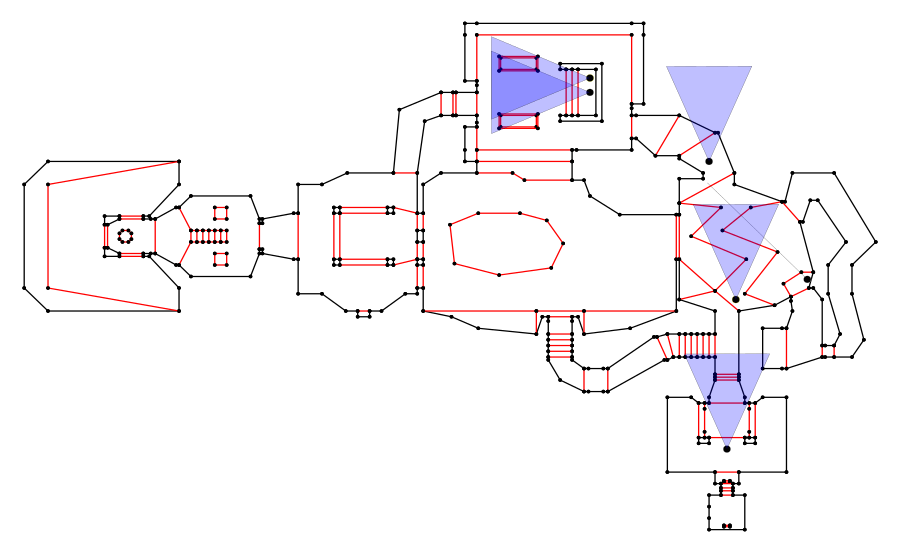
\includegraphics[width=\textwidth]{drawings/E1M1_sides.pdf}
\end{figure}
\par
Reject map based on enemies and monsters line of sight.\\


\pagebreak
\cfullimage{doombsp_compiling.png}{Building doombsp.}
\par
\cw{doombsp} generated several lumps and packaged them into a \cw{.wad} file\footnote{Explained on page XXX}.
\par
ARRAY OF LUMPS.
E1M1\\
THINGS\\
LINEDEFS\\
SIDEDEFS\\
VERTEXES\\
SEGS\\
SSECTORS\\
NODES\\
SECTORS\\
REJECT\\
BLOCKMAP\\
\par
\cfullimage{doombsp_run.png}{Running doombsp in debug mode show splitter selection.}
\par
